\documentclass[]{article}
\usepackage{lmodern}
\usepackage{amssymb,amsmath}
\usepackage{ifxetex,ifluatex}
\usepackage{fixltx2e} % provides \textsubscript
\ifnum 0\ifxetex 1\fi\ifluatex 1\fi=0 % if pdftex
  \usepackage[T1]{fontenc}
  \usepackage[utf8]{inputenc}
\else % if luatex or xelatex
  \ifxetex
    \usepackage{mathspec}
  \else
    \usepackage{fontspec}
  \fi
  \defaultfontfeatures{Ligatures=TeX,Scale=MatchLowercase}
\fi
% use upquote if available, for straight quotes in verbatim environments
\IfFileExists{upquote.sty}{\usepackage{upquote}}{}
% use microtype if available
\IfFileExists{microtype.sty}{%
\usepackage{microtype}
\UseMicrotypeSet[protrusion]{basicmath} % disable protrusion for tt fonts
}{}
\usepackage[margin=1in]{geometry}
\usepackage{hyperref}
\hypersetup{unicode=true,
            pdftitle={Meu primeiro documento em R Markdown},
            pdfauthor={Fernando Mayer},
            pdfborder={0 0 0},
            breaklinks=true}
\urlstyle{same}  % don't use monospace font for urls
\usepackage{color}
\usepackage{fancyvrb}
\newcommand{\VerbBar}{|}
\newcommand{\VERB}{\Verb[commandchars=\\\{\}]}
\DefineVerbatimEnvironment{Highlighting}{Verbatim}{commandchars=\\\{\}}
% Add ',fontsize=\small' for more characters per line
\usepackage{framed}
\definecolor{shadecolor}{RGB}{248,248,248}
\newenvironment{Shaded}{\begin{snugshade}}{\end{snugshade}}
\newcommand{\AlertTok}[1]{\textcolor[rgb]{0.94,0.16,0.16}{#1}}
\newcommand{\AnnotationTok}[1]{\textcolor[rgb]{0.56,0.35,0.01}{\textbf{\textit{#1}}}}
\newcommand{\AttributeTok}[1]{\textcolor[rgb]{0.77,0.63,0.00}{#1}}
\newcommand{\BaseNTok}[1]{\textcolor[rgb]{0.00,0.00,0.81}{#1}}
\newcommand{\BuiltInTok}[1]{#1}
\newcommand{\CharTok}[1]{\textcolor[rgb]{0.31,0.60,0.02}{#1}}
\newcommand{\CommentTok}[1]{\textcolor[rgb]{0.56,0.35,0.01}{\textit{#1}}}
\newcommand{\CommentVarTok}[1]{\textcolor[rgb]{0.56,0.35,0.01}{\textbf{\textit{#1}}}}
\newcommand{\ConstantTok}[1]{\textcolor[rgb]{0.00,0.00,0.00}{#1}}
\newcommand{\ControlFlowTok}[1]{\textcolor[rgb]{0.13,0.29,0.53}{\textbf{#1}}}
\newcommand{\DataTypeTok}[1]{\textcolor[rgb]{0.13,0.29,0.53}{#1}}
\newcommand{\DecValTok}[1]{\textcolor[rgb]{0.00,0.00,0.81}{#1}}
\newcommand{\DocumentationTok}[1]{\textcolor[rgb]{0.56,0.35,0.01}{\textbf{\textit{#1}}}}
\newcommand{\ErrorTok}[1]{\textcolor[rgb]{0.64,0.00,0.00}{\textbf{#1}}}
\newcommand{\ExtensionTok}[1]{#1}
\newcommand{\FloatTok}[1]{\textcolor[rgb]{0.00,0.00,0.81}{#1}}
\newcommand{\FunctionTok}[1]{\textcolor[rgb]{0.00,0.00,0.00}{#1}}
\newcommand{\ImportTok}[1]{#1}
\newcommand{\InformationTok}[1]{\textcolor[rgb]{0.56,0.35,0.01}{\textbf{\textit{#1}}}}
\newcommand{\KeywordTok}[1]{\textcolor[rgb]{0.13,0.29,0.53}{\textbf{#1}}}
\newcommand{\NormalTok}[1]{#1}
\newcommand{\OperatorTok}[1]{\textcolor[rgb]{0.81,0.36,0.00}{\textbf{#1}}}
\newcommand{\OtherTok}[1]{\textcolor[rgb]{0.56,0.35,0.01}{#1}}
\newcommand{\PreprocessorTok}[1]{\textcolor[rgb]{0.56,0.35,0.01}{\textit{#1}}}
\newcommand{\RegionMarkerTok}[1]{#1}
\newcommand{\SpecialCharTok}[1]{\textcolor[rgb]{0.00,0.00,0.00}{#1}}
\newcommand{\SpecialStringTok}[1]{\textcolor[rgb]{0.31,0.60,0.02}{#1}}
\newcommand{\StringTok}[1]{\textcolor[rgb]{0.31,0.60,0.02}{#1}}
\newcommand{\VariableTok}[1]{\textcolor[rgb]{0.00,0.00,0.00}{#1}}
\newcommand{\VerbatimStringTok}[1]{\textcolor[rgb]{0.31,0.60,0.02}{#1}}
\newcommand{\WarningTok}[1]{\textcolor[rgb]{0.56,0.35,0.01}{\textbf{\textit{#1}}}}
\usepackage{graphicx,grffile}
\makeatletter
\def\maxwidth{\ifdim\Gin@nat@width>\linewidth\linewidth\else\Gin@nat@width\fi}
\def\maxheight{\ifdim\Gin@nat@height>\textheight\textheight\else\Gin@nat@height\fi}
\makeatother
% Scale images if necessary, so that they will not overflow the page
% margins by default, and it is still possible to overwrite the defaults
% using explicit options in \includegraphics[width, height, ...]{}
\setkeys{Gin}{width=\maxwidth,height=\maxheight,keepaspectratio}
\IfFileExists{parskip.sty}{%
\usepackage{parskip}
}{% else
\setlength{\parindent}{0pt}
\setlength{\parskip}{6pt plus 2pt minus 1pt}
}
\setlength{\emergencystretch}{3em}  % prevent overfull lines
\providecommand{\tightlist}{%
  \setlength{\itemsep}{0pt}\setlength{\parskip}{0pt}}
\setcounter{secnumdepth}{5}
% Redefines (sub)paragraphs to behave more like sections
\ifx\paragraph\undefined\else
\let\oldparagraph\paragraph
\renewcommand{\paragraph}[1]{\oldparagraph{#1}\mbox{}}
\fi
\ifx\subparagraph\undefined\else
\let\oldsubparagraph\subparagraph
\renewcommand{\subparagraph}[1]{\oldsubparagraph{#1}\mbox{}}
\fi

%%% Use protect on footnotes to avoid problems with footnotes in titles
\let\rmarkdownfootnote\footnote%
\def\footnote{\protect\rmarkdownfootnote}

%%% Change title format to be more compact
\usepackage{titling}

% Create subtitle command for use in maketitle
\newcommand{\subtitle}[1]{
  \posttitle{
    \begin{center}\large#1\end{center}
    }
}

\setlength{\droptitle}{-2em}

  \title{Meu primeiro documento em R Markdown}
    \pretitle{\vspace{\droptitle}\centering\huge}
  \posttitle{\par}
    \author{Fernando Mayer}
    \preauthor{\centering\large\emph}
  \postauthor{\par}
      \predate{\centering\large\emph}
  \postdate{\par}
    \date{Abril, 2018}


\begin{document}
\maketitle

{
\setcounter{tocdepth}{2}
\tableofcontents
}
\hypertarget{sobre-o-markdown}{%
\section{Sobre o Markdown}\label{sobre-o-markdown}}

O Markdown é uma linguagem de marcação muito simples, desenvolvida por
John Gruber.

A ideia básica por trás da linguagem é fazer com que o escritor se
preocupe mais com o \textbf{conteúdo} do texto do que com a
\emph{formatação}.

Separe multiplas citações com \texttt{;}, por exemplo (Buckland et al.
2004; Valpine 2004).

Você pode adicionar comentários arbitrários dentro do colchetes, como
por exemplo (veja Durbin and Koopman 1997, 33--35; e Kitagawa 1987, cap.
1).

Remova os colchetes para criar citações no texto com Lele, Dennis, and
Lutscher (2007), ou Meinhold and Singpurwalla (2016, 5).

\hypertarget{mais-um-titulo}{%
\section{Mais um título}\label{mais-um-titulo}}

Aqui vamos tentar descrever uma análise.

\hypertarget{simulando-variaveis-aleatorias}{%
\section{Simulando variáveis
aleatórias}\label{simulando-variaveis-aleatorias}}

No R podemos simular valores de uma distribuição normal \[
f(x;\mu,\sigma^2) = \frac{1}{\sigma\sqrt{2\pi}}
e^{ -\frac{1}{2}\left(\frac{x-\mu}{\sigma}\right)^2 }
\] através da função \texttt{rnorm()}.

Seja \(X \sim \text{N}(0,1)\), então para gerar 30 valores dessa
variável aleatório normal, fazemos

\begin{Shaded}
\begin{Highlighting}[]
\NormalTok{(x <-}\StringTok{ }\KeywordTok{rnorm}\NormalTok{(}\DecValTok{30}\NormalTok{))}
\end{Highlighting}
\end{Shaded}

\begin{verbatim}
##  [1]  0.39845268 -1.26818768  1.09788250 -0.07442224 -0.39461864
##  [6]  0.73382703  1.17292910  0.56899170 -0.40996614 -1.02448086
## [11] -0.88470208 -0.42488088  0.48988737 -0.31623555 -1.69747103
## [16] -2.20704638 -0.61833971  0.27008219 -0.07446170 -1.37495426
## [21]  2.17923437  0.14290015 -3.47975609 -0.36278608  1.25929414
## [26] -0.43179901 -2.08859075 -0.15821341 -0.12960261  0.84157247
\end{verbatim}

\hypertarget{comentarios}{%
\subsection{Comentários}\label{comentarios}}

Com o resultado dessa simulação, podemos calcular a média e a variância
dessa VA \(X\) para conferir se o resultado fica próximo de 0 e 1,
respectivamente.

Nessa simulação, a média resultou em -0.2755154 e a variância em
1.3659802.

\hypertarget{visualizacao}{%
\section{Visualização}\label{visualizacao}}

Também podemos fazer um histograma dessa VA \(X\) simulada

\begin{Shaded}
\begin{Highlighting}[]
\KeywordTok{hist}\NormalTok{(x)}
\end{Highlighting}
\end{Shaded}

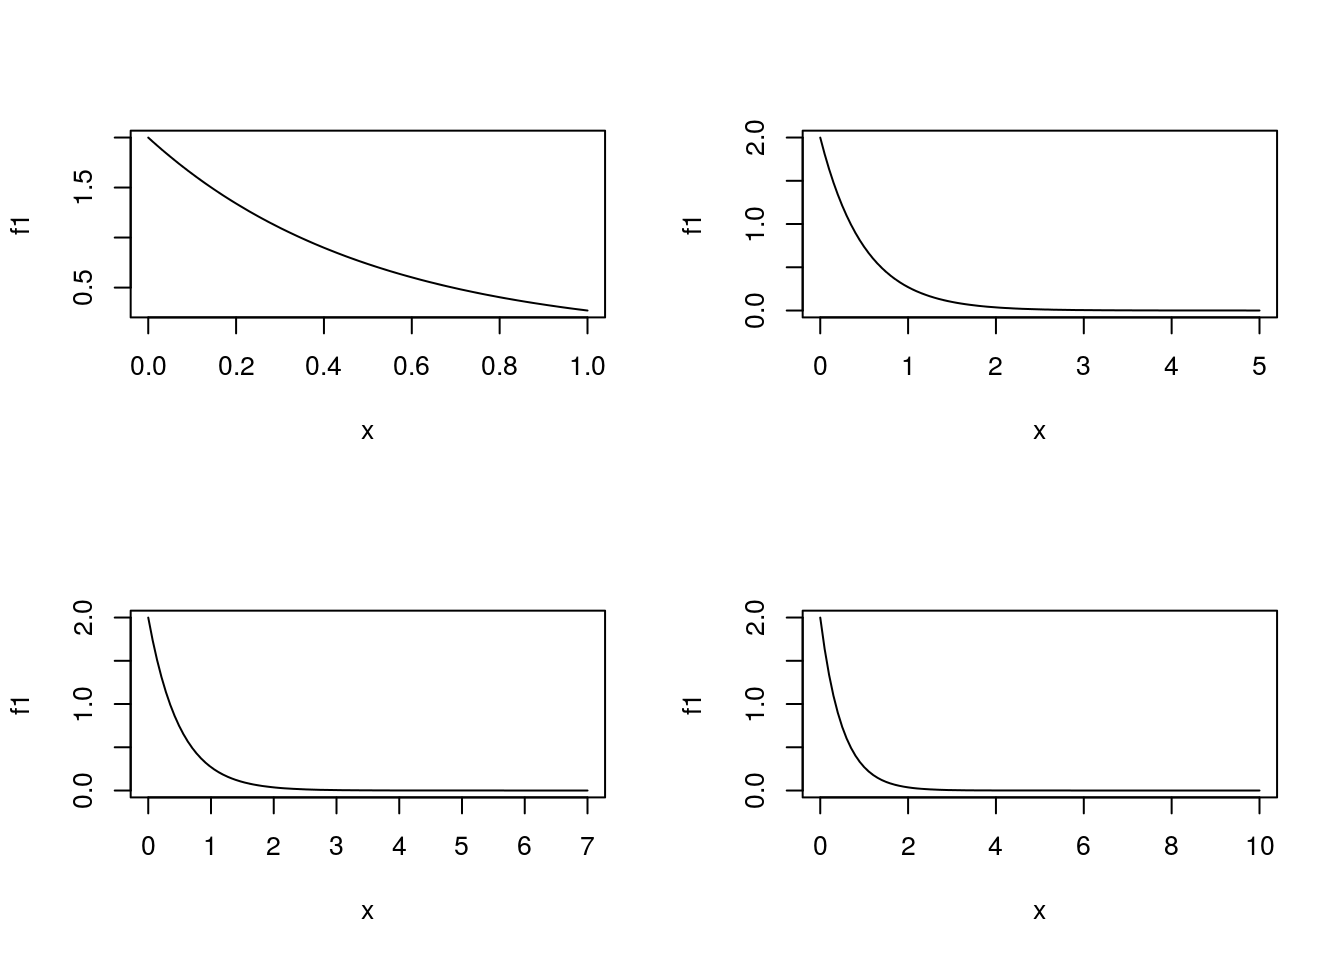
\includegraphics{Exemplo3-knitr_files/figure-latex/unnamed-chunk-2-1.pdf}

\hypertarget{referencias}{%
\section*{Referências}\label{referencias}}
\addcontentsline{toc}{section}{Referências}

\hypertarget{refs}{}
\leavevmode\hypertarget{ref-Buckland2004}{}%
Buckland, S.T., K.B. Newman, L. Thomas, and N.B. Koesters. 2004.
``State-space models for the dynamics of wild animal populations.''
\emph{Ecological Modelling} 171 (1-2):157--75.
\url{https://doi.org/10.1016/j.ecolmodel.2003.08.002}.

\leavevmode\hypertarget{ref-Durbin1997}{}%
Durbin, J., and S. Koopman. 1997. ``Monte Carlo maximum likelihood
estimation for non-Gaussian state space models.'' \emph{Biometrika} 84
(3):669--84. \url{http://eprints.ucl.ac.uk/18394/}.

\leavevmode\hypertarget{ref-Kitagawa1987}{}%
Kitagawa, G. 1987. ``Non-Gaussian State-Space Modeling on Nonstationary
Time Series.'' \emph{Journal of the American Statistical Association} 82
(400):1032--63.

\leavevmode\hypertarget{ref-Lele2007}{}%
Lele, Subhash R, Brian Dennis, and Frithjof Lutscher. 2007. ``Data
cloning: easy maximum likelihood estimation for complex ecological
models using Bayesian Markov chain Monte Carlo methods.'' \emph{Ecology
Letters} 10 (7):551--63.
\url{https://doi.org/10.1111/j.1461-0248.2007.01047.x}.

\leavevmode\hypertarget{ref-Meinhold2016}{}%
Meinhold, Richard J, and Nozer D Singpurwalla. 2016. ``Understanding the
Kalman Filter.'' \emph{The American Statistician} 37 (2):123--27.

\leavevmode\hypertarget{ref-DeValpine2004}{}%
Valpine, Perry de. 2004. ``Monte Carlo State-Space Likelihoods by
Weighted Posterior Kernel Density Estimation.'' \emph{Journal of the
American Statistical Association} 99 (466):523--36.
\url{https://doi.org/10.1198/016214504000000476}.


\end{document}
